\documentclass{svproc}

\usepackage{url}
\def\UrlFont{\rmfamily}
\usepackage{amsmath}
\usepackage{amssymb}
\usepackage{graphicx}
\usepackage{booktabs}
\usepackage{microtype}
\usepackage{array}
\usepackage[numbers,sort&compress]{natbib}

% Graphicspath setup for Overleaf and local compilation
\graphicspath{{paper_figs/final/}{../paper_figs/final/}{./}}

\begin{document}
\mainmatter

\title{Squared Sense: Multi-Scale 3D Voxel World Modeling with Event-Driven Shell Gating and Dual-LSTM Temporal Integration}

\titlerunning{Squared Sense: Multi-Scale 3D Voxel World Modeling}

\author{Aryan Mishra\inst{1}\thanks{Corresponding author: \email{aryan.mishra@institution.edu}} \and Co-Author Name\inst{1}}

\authorrunning{Aryan Mishra et al.}

\institute{Department of Computer Science, Institution Name, City, Country\\
\email{aryan.mishra@institution.edu}}

\maketitle

\begin{abstract}
Embodied artificial intelligence agents operating in visually complex, open-world three-dimensional (3D) environments such as Minecraft face a persistent tension between sensory resolution and spatial horizon. While two-dimensional RGB observations suffer from depth ambiguity and lighting variance, uniform 3D voxel representations scale cubically with volume, constraining real-time perception. In this work, we present Squared Sense, an egocentric world modeling framework built upon concentric, multi-Level-of-Detail (multi-LOD) 3D voxel shells. Our architecture couples a Siamese 3D ConvNeXt encoder with a self-supervised Spatial Joint-Embedding Predictive Architecture (Spatial JEPA) regularized by Variance-Invariance-Covariance Regularization (VICReg), learning invariant geometric latents without generative pixel reconstruction. To achieve high operational efficiency, an event-driven shell gating mechanism evaluates temporal voxel differences, selectively skipping convolutional and transformer passes for static shells. A Dual-LSTM temporal integrator couples spatial memory slots with proprioceptive agent telemetry through differentiable trilinear 3D ego-motion shift and query cross-attention, predicting future latents over multi-step discounted rollouts alongside an auxiliary inverse dynamics model. Evaluated across frozen probe suites and closed-loop reinforcement learning navigation in a simulated voxel physics environment, Squared Sense provides a grounded foundation for embodied spatial intelligence.
\keywords{Embodied AI, World Models, Joint-Embedding Predictive Architecture, 3D Voxel Perception, Event-Driven Gating, Recurrent Dynamics}
\end{abstract}

\section{Introduction}

Embodied artificial intelligence agents deployed in complex 3D virtual worlds must maintain accurate, predictive representations of their surrounding geometry to navigate, avoid environmental hazards, and pursue long-horizon objectives~\cite{hafner2023dreamerv3,baker2022vpt}. In open-ended voxel domains such as Minecraft~\cite{guss2019minerl,fan2022minedojo}, standard agents predominantly process egocentric two-dimensional (2D) RGB video streams. Although visual transformers and convolutional networks have achieved notable successes in imitation learning and reinforcement learning (RL) from human gameplay demonstrations~\cite{baker2022vpt}, pure pixel-based observation remains susceptible to monocular depth ambiguities, camera viewpoint jitter, perspective foreshortening, and severe visual distractions such as dynamic weather, underwater lighting shifts, and night illumination drop-off. 

Direct 3D voxel perception resolves these geometric ambiguities by encoding explicit spatial occupancy and physical affordance semantics. However, uniform 3D voxel grids suffer from an acute spatial-horizon versus resolution dilemma driven by cubic volumetric scaling $\mathcal{O}(L^3)$. Fine obstacle avoidance—such as stepping over a 1-block lava pool, detecting open cliff edges, or ascending stairs—demands single-block metric resolution ($1\times1\times1$ blocks). Conversely, long-range topological navigation, visual beacon alignment, and target tracking require spatial horizons extending across dozens of blocks. A uniform high-resolution voxel grid covering an egocentric volume of $64\times64\times64$ blocks contains $262{,}144$ voxels; processing such tensors at typical simulation control frequencies ($5\text{--}20\text{ Hz}$) incurs severe memory and computational overhead, exceeding the edge compute budgets typical of robotic or local agent deployments.

To overcome this volumetric bottleneck, we introduce \textbf{Squared Sense}, an efficient, self-supervised 3D world modeling architecture. Squared Sense establishes an egocentric, multi-scale sensory framework via three nested, concentric Level-of-Detail (multi-LOD) voxel shells. Each shell covers a distinct spatial span ($16^3$, $32^3$, and $64^3$ blocks) downsampled onto a fixed $16\times16\times16$ tensor grid, combining cardinal yaw-snapping with rotational hysteresis and pitch-dependent vertical anchor shift. To learn representations without generative voxel decoding, we formulate a non-generative \textbf{Spatial Joint-Embedding Predictive Architecture (Spatial JEPA)} based on the joint-embedding paradigm of LeCun~\cite{assran2023ijepa}. Trained with 3D block-structured masking, an Exponential Moving Average (EMA) target encoder, and Variance-Invariance-Covariance Regularization (VICReg)~\cite{bardes2022vicreg}, our Siamese 3D ConvNeXt backbone learns expressive latent representations that resist dimensional collapse without contrastive negative pairs.

Furthermore, we observe that during locomotion in 3D environments, outer spatial shells exhibit high temporal redundancy across successive frames compared to immediate near-field voxels. Exploiting this spatial-temporal asymmetry, we develop an \textbf{Event-Driven Shell Gate} that monitors temporal $L_1$ voxel differences against a calibrated threshold $\tau_{\text{gate}}$. This mechanism selectively skips 3D convolutional encoding on quiescent shells and completely bypasses the multi-LOD Transformer when no volumetric change is registered, substantially lowering inference latency. Finally, we formulate a \textbf{Dual-LSTM Temporal Integrator} that unrolls spatial memory over time, explicitly compensating for agent translation via differentiable trilinear 3D ego-motion coordinate shifting, fusing proprioceptive state telemetry via query cross-attention, and training against multi-step autoregressive latent rollouts and auxiliary inverse dynamics.

This work delivers four primary contributions:
\begin{enumerate}
    \item \textbf{Concentric Multi-LOD Voxel Representation:} A hierarchical, 16-channel egocentric representation combining asymmetric bounding boxes, cardinal hysteresis snapping, and salience-preserving max/average pooling, balancing near-field precision with far-field horizon.
    \item \textbf{Self-Supervised Spatial JEPA with VICReg:} A 4.65M-parameter Siamese 3D ConvNeXt and Pre-LN Transformer architecture pre-trained via 3D block masking and non-contrastive covariance regularization, provably preserving representation rank without negative pairs.
    \item \textbf{Zero-Parameter Event-Driven Shell Gating:} An inference-time temporal difference gating mechanism that yields up to $60.2\%$ empirical compute reduction by selectively evaluating only dynamic voxel shells.
    \item \textbf{Ego-Motion-Compensated Dual-LSTM Dynamics:} A temporal integrator incorporating trilinear coordinate shifting across multi-scale volumes, verified through a rigorous suite of frozen linear/MLP probes and closed-loop reinforcement learning navigation.
\end{enumerate}

\section{Related Work}

\subsection{3D Voxel Representations for Embodied Agents}
Spatial perception in embodied environments historically relies on occupancy grids, point clouds, or octrees~\cite{ha2018worldmodels,wang2023voyager}. In robotic mapping, octrees compress sparse free space but introduce non-uniform pointer dereferencing, irregular memory access, and branch divergence that hinder vectorized execution on SIMD tensor accelerators. Uniform dense voxel grids, while hardware-friendly, scale cubically with spatial diameter, forcing agents to operate within cramped local bounding boxes. Recent large-scale Minecraft agents such as Video PreTraining (VPT)~\cite{baker2022vpt} and MineDojo~\cite{fan2022minedojo} circumvent volumetric costs by relying exclusively on 2D RGB frames. However, such agents demand thousands of GPU hours and millions of human demonstration frames to implicitly disentangle spatial depth from visual textures. Squared Sense bridges this divide by enforcing uniform dense tensor dimensions ($16\times16\times16$) across nested concentric shells, retaining full hardware tensor acceleration while providing logarithmic spatial horizon expansion.

\subsection{Self-Supervised World Models and Joint-Embedding Predictive Architectures}
World models enable embodied agents to anticipate the consequences of actions within internal latent dynamics models~\cite{ha2018worldmodels,hafner2023dreamerv3}. Canonical architectures like DreamerV3~\cite{hafner2023dreamerv3} rely on generative reconstruction via autoencoders or discrete vector-quantized codebooks. However, pixel reconstruction forces models to allocate significant capacity to unpredictable or irrelevant high-frequency textures rather than underlying geometric affordances. 

As articulated in LeCun's vision for autonomous machine intelligence~\cite{lecun2022path}, Joint-Embedding Predictive Architectures (JEPAs) circumvent generative decoding by performing predictions exclusively in abstract latent feature space. Prominent implementations including I-JEPA~\cite{assran2023ijepa} for images and V-JEPA~\cite{bardes2024vjepa} for video patches demonstrate that masking contiguous spatiotemporal regions and predicting target representations from context tokens yields semantically structured representations. To avoid representational collapse where all inputs map to a trivial constant vector, early self-supervised systems relied on contrastive negative pairs or heuristic stop-gradient momentum updates~\cite{grill2020byol}. Non-contrastive approaches like Barlow Twins~\cite{zbontar2021barlow} and VICReg~\cite{bardes2022vicreg} explicitly constrain variance and penalize off-diagonal covariance across embedding dimensions. The uncentered RankMe metric~\cite{garrido2023rankme} provides an effective tool to quantify continuous representation dimensionality without thresholding singular values. Squared Sense extends the JEPA paradigm to multi-scale 3D concentric voxel volumes, providing a spatial counterpart to temporal hierarchical architectures such as H-JEPA~\cite{lecun2022path}, while contrasting directly with generative Masked Autoencoders (3D-MAE)~\cite{he2022mae}.

\subsection{Embodied Agents and Navigation in Minecraft}
Minecraft has emerged as a landmark challenge for reinforcement learning, offering open-world survival, sparse rewards, and dynamic terrain~\cite{guss2019minerl,fan2022minedojo,wang2023voyager}. Previous efforts have explored hierarchical reinforcement learning, visual language planning, and large-scale behavioral cloning~\cite{baker2022vpt,wang2023voyager}. Nonetheless, navigation over hazardous, procedurally generated terrain remains hazardous for pixel-trained agents due to texture variation, fog, and underwater occlusion. By utilizing local voxel crops directly derived from world memory, Squared Sense grounds policy learning in explicit geometry, enabling lightweight actor-critic architectures to solve challenging navigation tasks without ungrounded visual hallucinations.

\section{Methodology}

\subsection{Multi-LOD Concentric Voxel Schema}
The input space of Squared Sense is defined as a concentric hierarchy of three 3D voxel shells centered on the agent, denoted by $l \in \{0, 1, 2\}$. Each shell has a fixed spatial dimension of $16 \times 16 \times 16$ voxels across 16 semantic channels, represented as a channel-last tensor $\mathbf{X}_l \in \mathbb{R}^{16 \times 16 \times 16 \times 16}$. Across all three shells, the composite input tensor is $\mathbf{X} \in \mathbb{R}^{3 \times 16 \times 16 \times 16 \times 16}$, normalized from raw disk bytes $u \in \{0, \dots, 255\}$ to unit floats $x \in [0.0, 1.0]$ via $x = u / 255.0$.

Each shell level scales geometrically by $s_l = 2^l \in \{1, 2, 4\}$. To prioritize the agent's forward path while retaining rear awareness, each shell occupies an asymmetric egocentric bounding box:
\begin{itemize}
    \item \textbf{LOD-0 ($s_0 = 1\times$):} $16^3$ span; forward $+12$, back $-4$, lateral $\pm 8$, vertical $Y \in [-4, +12]$.
    \item \textbf{LOD-1 ($s_1 = 2\times$):} $32^3$ span; forward $+24$, back $-8$, lateral $\pm 16$, vertical $Y \in [-8, +24]$.
    \item \textbf{LOD-2 ($s_2 = 4\times$):} $64^3$ span; forward $+48$, back $-16$, lateral $\pm 32$, vertical $Y \in [-16, +48]$.
\end{itemize}

\begin{table}[t]
\centering
\caption{Semantic 16-channel voxel schema and spatial pooling partitions}
\label{tab:schema}
\begin{tabular}{c l l c}
\toprule
\textbf{Channel} & \textbf{Semantic Class} & \textbf{Physical Definition / Value Range} & \textbf{Pooling Rule} \\
\midrule
0 & Terrain & Solid, opaque walkable ground blocks & Average \\
1 & Air & Passable empty space & Average \\
2 & Hazard & Active hazards (lava, fire, magma blocks) & Maximum \\
3 & Liquid & Passable fluids (water) & Average \\
4 & Climbable & Vertical transit structures (ladders, vines) & Maximum \\
5 & Foliage & Non-solid fragile blocks (grass, leaves) & Average \\
6 & World Y & Normalized vertical coordinate in $[-64, 320]$ & Average \\
7 & Collision Height & Fractional bounding box height ($0\text{--}255$) & Maximum \\
8 & Waypoint & Goal beacon or navigation marker & Maximum \\
9 & Resource & Interactive or minable resource block & Maximum \\
10 & Walkable Surface & Solid block directly below $\ge 2$ air blocks & Maximum \\
11 & Light Level & Combined sky and block light: $\max(\text{sky}, \text{block})/15$ & Average \\
12 & Lethal Drop & Cliff boundary with fall drop $\ge 3$ blocks & Maximum \\
13 & Surface Shell & Boundary voxel between solid terrain and air & Maximum \\
14 & Block Hardness & Normalized mining break time ($0.0\text{--}1.0$) & Average \\
15 & Out-of-Bounds & Void padding mask outside course boundary & Maximum \\
\bottomrule
\end{tabular}
\end{table}

To prevent continuous micro-rotations from constantly triggering voxel reslicing, we employ cardinal yaw-snapping with rotational hysteresis. The agent yaw $\psi \in [0, 360^\circ)$ is snapped to the nearest cardinal axis $\psi_{\text{card}} \in \{0^\circ, 90^\circ, 180^\circ, 270^\circ\}$. The snapped heading is retained until the angular deviation exceeds a deadband threshold of $|\psi - \psi_{\text{card}}| > 60^\circ$ ($\pm 15^\circ$ past intermediate diagonals). Pitch adjustments vertically shift the observation window according to:
\begin{equation}
\Delta y_l = \mathrm{round}\left(4 \sin \theta\right) \cdot s_l,
\end{equation}
where $\theta$ denotes the camera pitch angle in radians and $s_l$ is the shell scale. 

Downsampling from larger world volumes onto the $16 \times 16 \times 16$ grid requires pooling that preserves both structural continuity and critical hazards. As defined in Table~\ref{tab:schema}, channels are partitioned into disjoint sets: continuous volumetric fields (e.g., air, terrain density, world height, light) undergo average pooling, whereas sparse, safety-critical features (e.g., lava, cliffs, climbables, waypoints) undergo maximum pooling to preserve their salience under spatial coarsening.

\subsection{Siamese 3D ConvNeXt Encoder and Spatial JEPA}
Each voxel shell $\mathbf{X}_l \in \mathbb{R}^{16 \times 16 \times 16 \times 16}$ is initially processed by a CoordConv3D module~\cite{liu2018coordconv}. This layer appends a static, non-trainable 3D meshgrid $(u, v, w) \in [-1, 1]^3$ along the channel dimension, producing an augmented tensor of shape $16 \times 16 \times 16 \times 19$. 

A shared Siamese 3D ConvNeXt encoder~\cite{liu2022convnet} extracts latent tokens from each shell. The architecture employs a stem convolution ($2\times2\times2$ kernel, stride 2, valid padding, LayerNorm~\cite{ba2016layernorm}) yielding feature maps of shape $8\times8\times8\times64$. This is followed by Stage 1, consisting of two ConvNeXt-3D blocks with Squeeze-and-Excitation (SE) channel attention~\cite{hu2018squeeze}. Each block applies depthwise $3\times3\times3$ convolutions (grouped by channels), LayerNorm, a pointwise MLP with GELU activations expanding channels $64 \to 256 \to 64$, and an SE reduction factor of 4. A downsampling convolution ($2\times2\times2$, stride 2) compresses the representation to $4\times4\times4\times128$, followed by Stage 2 containing two ConvNeXt-3D blocks at dimension 128. Finally, a $1\times1\times1$ convolution projects the feature dimension to 256, flattening the spatial volume into $4^3 = 64$ tokens per shell:
\begin{equation}
\mathbf{T}_l = \mathrm{Flatten}\left(\mathrm{Conv3D}_{1\times1\times1}\left(\mathbf{H}_l^{(2)}\right)\right) \in \mathbb{R}^{64 \times 256}.
\end{equation}
Across three concentric shells, this yields $3 \times 64 = 192$ spatial tokens $\mathbf{T} \in \mathbb{R}^{B \times 192 \times 256}$.

Before transformer processing, we inject structured geometric information via additive learnable embeddings: a spatial coordinate embedding $\mathbf{E}_{\text{spatial}} \in \mathbb{R}^{1 \times 1 \times 64 \times 256}$ shared across shells, and a scale embedding $\mathbf{E}_{\text{scale}} \in \mathbb{R}^{1 \times 3 \times 1 \times 256}$ identifying the LOD level:
\begin{equation}
\mathbf{T}_{\text{pos}} = \mathbf{T} + \left(\mathbf{E}_{\text{spatial}} \oplus \mathbf{E}_{\text{scale}}\right).
\end{equation}

For self-supervised pre-training, we employ 3D block-structured masking. Each shell's $4 \times 4 \times 4$ token volume is partitioned into 8 disjoint $2 \times 2 \times 2$ blocks ($8$ tokens each). For each shell, 4 blocks ($32$ tokens) are sampled as prediction targets, while the remaining 4 blocks ($32$ tokens) serve as visible context, yielding $N_{\text{vis}} = 96$ visible tokens and $N_{\text{tgt}} = 96$ target tokens across the three shells. To force the model to integrate multi-scale context, we apply cross-scale complementary masking with probability $p = 0.3$: when active, target blocks in LOD-0 are forced to be visible in LOD-1 and LOD-2, requiring the network to leverage coarser shells to resolve fine local geometry.

The context encoder, parameterized by a 4-layer Pre-LN Transformer~\cite{vaswani2017attention} ($D = 256, H = 8, \text{mlp} = 4$), processes only the gathered visible tokens:
\begin{equation}
\mathbf{U}_{\text{vis}} = \mathrm{Transformer}_{\text{ctx}}\left(\mathbf{T}_{\text{pos}}[\mathcal{I}_{\text{vis}}]\right) \in \mathbb{R}^{B \times 96 \times 256}.
\end{equation}
The JEPA Predictor is a lightweight 2-layer Pre-LN Transformer ($D = 192, H = 6$). It projects $\mathbf{U}_{\text{vis}}$ from dimension 256 to 192 via a linear layer, appends predictor positional embeddings, and concatenates learnable mask query tokens at target positions $\mathcal{I}_{\text{tgt}}$:
\begin{equation}
\mathbf{Q}_{\text{pred}} = \left[\mathbf{W}_{\text{in}}\mathbf{U}_{\text{vis}} + \mathbf{E}_{\text{pred}}[\mathcal{I}_{\text{vis}}]\,;\,\mathbf{e}_{\text{mask}} + \mathbf{E}_{\text{pred}}[\mathcal{I}_{\text{tgt}}]\right] \in \mathbb{R}^{B \times 192 \times 192}.
\end{equation}
After propagating through the predictor blocks, the target token positions are extracted and linearly projected back to dimension 256, yielding predicted latents $\hat{\mathbf{S}} \in \mathbb{R}^{B \times 96 \times 256}$.

The target representations $\tilde{\mathbf{S}}$ are generated by an identical target encoder whose parameters $\theta_{\text{tgt}}$ are updated via an Exponential Moving Average (EMA) of context parameters $\theta_{\text{ctx}}$:
\begin{equation}
\theta_{\text{tgt}} \leftarrow m_t \theta_{\text{tgt}} + (1 - m_t) \theta_{\text{ctx}},
\end{equation}
where $m_t$ follows a cosine schedule increasing from $0.996$ to $1.0$ over training steps. The target encoder processes the unmasked voxel shells under $\mathrm{stop\_gradient}$. Target tokens at indices $\mathcal{I}_{\text{tgt}}$ are normalized per-token via LayerNorm: $\tilde{\mathbf{s}} = (\mathbf{s} - \mu) / \sqrt{\sigma^2 + 10^{-6}}$.

The Spatial JEPA objective combines Smooth-L1 latent prediction error with VICReg regularization~\cite{bardes2022vicreg} on visible context representations $\mathbf{U}_{\text{vis}}$:
\begin{equation}
\mathcal{L}_{\text{spatial}} = \mathcal{L}_{\text{pred}}\left(\hat{\mathbf{S}}, \tilde{\mathbf{S}}\right) + \alpha \mathcal{L}_{\text{var}}\left(\mathbf{U}_{\text{vis}}\right) + \beta \mathcal{L}_{\text{cov}}\left(\mathbf{U}_{\text{vis}}\right),
\end{equation}
where $\alpha = 0.1$ and $\beta = 0.04$. The prediction loss is the mean Huber error with transition parameter $\beta_{\text{huber}} = 1.0$:
\begin{equation}
\mathcal{L}_{\text{pred}}(\mathbf{x}, \mathbf{y}) = \frac{1}{|\mathbf{x}|} \sum_i \begin{cases} 
0.5 (x_i - y_i)^2, & \text{if } |x_i - y_i| < 1.0, \\ 
|x_i - y_i| - 0.5, & \text{otherwise}. 
\end{cases}
\end{equation}
The VICReg penalties prevent representational collapse without contrastive negative pairs:
\begin{equation}
\mathcal{L}_{\text{var}}(\mathbf{Z}) = \frac{1}{D} \sum_{j=1}^D \max\left(0, 1.0 - \sqrt{\mathrm{Var}(\mathbf{z}_j) + 10^{-4}}\right),
\end{equation}
\begin{equation}
\mathcal{L}_{\text{cov}}(\mathbf{Z}) = \frac{1}{D} \sum_{j \neq k} \mathbf{C}_{j,k}^2, \quad \text{where } \mathbf{C} = \frac{1}{N - 1} (\mathbf{Z} - \bar{\mathbf{Z}})^T (\mathbf{Z} - \bar{\mathbf{Z}}).
\end{equation}

\subsection{Event-Driven Shell Gating}
During real-time deployment, the agent frequently experiences stationary states or straight-line translation where outer shells change slowly due to spatial coarsening. We introduce a zero-parameter Event-Driven Shell Gate that monitors the mean absolute voxel change for each shell:
\begin{equation}
\delta_{t, l} = \frac{1}{|V|} \sum_{x,y,z,c} \left| \mathbf{X}_{t, l}(x,y,z,c) - \mathbf{X}_{t-1, l}(x,y,z,c) \right|.
\end{equation}
If $\delta_{t, l} \le \tau_{\text{gate}}$ (with default threshold $\tau_{\text{gate}} = 0.05$), shell $l$ bypasses the Siamese 3D ConvNeXt, and its cached token representation $\mathbf{T}_{t-1, l}$ is reused. If all three shells satisfy $\delta_{t, l} \le \tau_{\text{gate}}$, the multi-LOD Transformer is entirely skipped, returning the previous step's latent representation $\mathbf{Z}_{t-1}$:
\begin{equation}
\mathbf{Z}_t = \begin{cases}
\mathbf{Z}_{t-1}, & \text{if } \max_{l} \delta_{t, l} \le \tau_{\text{gate}}, \\
\mathrm{Transformer}\left(\left[\hat{\mathbf{T}}_{t,0}\,;\,\hat{\mathbf{T}}_{t,1}\,;\,\hat{\mathbf{T}}_{t,2}\right]\right), & \text{otherwise},
\end{cases}
\end{equation}
where $\hat{\mathbf{T}}_{t,l} = \mathrm{CNN}(\mathbf{X}_{t,l})$ if $\delta_{t,l} > \tau_{\text{gate}}$ else $\mathbf{T}_{t-1,l}$. Because outer shells cover large physical extents ($64^3$ blocks), a single block movement alters only a tiny fraction of their downsampled volume, enabling outer shells to skip evaluation significantly more often than LOD-0.

\subsection{Dual-LSTM Temporal Integrator with 3D Ego-Motion Shift}
To model physical dynamics across time, spatial tokens are first average-pooled from $4 \times 4 \times 4$ down to $2 \times 2 \times 2$ blocks per shell, producing 24 coarse spatial slots:
\begin{equation}
\mathbf{M}_t = \mathrm{Pool}_{2\times2\times2}(\mathbf{T}_t) \in \mathbb{R}^{B \times 24 \times 256}.
\end{equation}
When the agent translates by displacement $\Delta \mathbf{p} = (\Delta x, \Delta y, \Delta z)$ extracted from telemetry $\mathbf{s}_t[3:6]$, the spatial coordinates of the agent's memory must shift in the opposite direction. We apply a differentiable 3D ego-motion shift to the spatial hidden state $\mathbf{h}_{\text{sp}} \in \mathbb{R}^{B \times 3 \times 2 \times 2 \times 2 \times 192}$:
\begin{equation}
\mathbf{h}_{\text{sp}, l}^{\text{shifted}} = \mathrm{map\_coordinates}\left(\mathbf{h}_{\text{sp}, l},\, \mathbf{c}_{\text{base}} + \frac{\Delta \mathbf{p}}{8.0 \cdot s_l},\, \text{order}=1\right),
\end{equation}
where trilinear interpolation is vectorized across spatial and channel axes with constant zero boundary padding. The shifted slots are updated by a shared `Spatial LSTM` ($256 \to 192$):
\begin{equation}
\mathbf{h}_{\text{sp}, t}, \mathbf{c}_{\text{sp}, t} = \mathrm{LSTM}_{\text{sp}}\left(\mathbf{M}_t,\, (\mathbf{h}_{\text{sp}, t-1}^{\text{shifted}}, \mathbf{c}_{\text{sp}, t-1}^{\text{shifted}})\right).
\end{equation}

Concurrently, a `State LSTM` ($12 \to 64$) ingests the 12-dimensional proprioceptive vector $\mathbf{s}_t$ (velocities, displacements, heading sines/cosines, pitch, health, food, grounded flag), projected linearly ($64 \to 192$) to form a state query token $\mathbf{q}_t \in \mathbb{R}^{B \times 1 \times 192}$. A Pre-LN Query Cross-Attention block ($H = 6, D = 192$) queries the 24 spatial memory slots with $\mathbf{q}_t$:
\begin{equation}
\mathbf{c}_t = \mathrm{CrossAttention}\left(\mathbf{q}_t,\, \mathbf{h}_{\text{sp}, t}\right) \in \mathbb{R}^{B \times 192}.
\end{equation}

Conditioned on the discrete action embedding $\mathbf{a}_t \in \mathbb{R}^{64}$, a forward predictor MLP ($256 \to 192 \to 256$) predicts the next-step pooled latent:
\begin{equation}
\hat{\mathbf{z}}_{t+1} = \mathrm{MLP}_{\text{fwd}}\left(\left[\mathbf{c}_t\,;\,\mathbf{a}_t\right]\right) \in \mathbb{R}^{B \times 256}.
\end{equation}
The network is unrolled over $K = 4$ steps with discount $\gamma_{\text{discount}} = 0.9$. An auxiliary Inverse Dynamics Model (IDM) predicts the action from consecutive latents $[\mathbf{z}_t\,;\,\mathbf{z}_{t+1}] \in \mathbb{R}^{512} \to \mathbb{R}^{12}$:
\begin{equation}
\mathcal{L}_{\text{temporal}} = \frac{1}{K} \sum_{k=1}^K \gamma^{k-1} \|\hat{\mathbf{z}}_{t+k} - \mathbf{z}_{t+k}\|_1 + \omega \mathcal{L}_{\text{CE}}(\hat{\mathbf{a}}_t, \mathbf{a}_t) + \alpha \mathcal{L}_{\text{var}} + \beta \mathcal{L}_{\text{cov}},
\end{equation}
with IDM weight $\omega = 0.2$. Optimization is performed using AdamW~\cite{loshchilov2019adamw} (weight decay $0.05$) under a two-phase schedule: Phase 1 (15 epochs) trains only the Dual-LSTM with frozen spatial representations at learning rate $3 \times 10^{-4}$; Phase 2 (25 epochs) unfreezes the top two transformer blocks of the context encoder at $0.1\times$ learning rate ($3 \times 10^{-5}$) with a spatial anchoring penalty.

\section{Experimental Setup}

\subsection{Real-World Minecraft Dataset and Course Generation}
Trajectory episodes are extracted from offline Minecraft Anvil `.mca` world archives logged at $5\text{ Hz}$. Each sample comprises voxel shells $\mathbf{X} \in \mathbb{R}^{T \times 3 \times 16 \times 16 \times 16 \times 16}$, proprioceptive states $\mathbf{s} \in \mathbb{R}^{T \times 12}$, discrete actions $a \in \{0, \dots, 11\}^T$, and metadata $\mathbf{m} \in \mathbb{R}^{T \times 6}$. Trajectories are split deterministically at the episode level into $70\%$ training, $15\%$ validation, and $15\%$ testing sets, strictly avoiding frame-level leakage.

Closed-loop navigation is evaluated in the custom `VoxelNavEnv` simulator, operating over course volumes of shape $16 \times 128 \times 64 \times 128$ voxels. The agent executes 12 discrete actions: translation (Forward, Back, Left, Right), combined maneuvers (Forward-Left, Forward-Right, Step-Up-Forward), turning ($\pm 45^\circ$), pitch adjustment ($\pm 15^\circ$), and idle. Physics rules enforce 1-block vertical step-ups, penalize drops $\ge 3$ blocks, and terminate episodes upon entering hazards ($ch_2 \ge 128$). Distance-to-goal potential shaping is combined with time penalties.

\subsection{Parameter-Matched Baselines and Ablations}
We benchmark five parameter-matched architectural configurations:
\begin{itemize}
    \item \textbf{M1 (Full Squared Sense):} Spatial JEPA encoder ($3.65\text{M}$) with Dual-LSTM ($0.72\text{M}$); $5.37\text{M}$ parameters during training, $4.37\text{M}$ at inference.
    \item \textbf{M2 (Static Spatial JEPA):} Multi-LOD Spatial JEPA backbone ($3.65\text{M}$) without recurrent temporal integration.
    \item \textbf{B1 (Single-LOD0 JEPA):} Spatial JEPA trained exclusively on the high-resolution near-field shell ($1\times$ scale, 64 tokens, $4.65\text{M}$ params).
    \item \textbf{B2 (Single-LOD2 JEPA):} Spatial JEPA trained exclusively on the coarse far-field shell ($4\times$ scale, 64 tokens, $4.65\text{M}$ params).
    \item \textbf{B3 (Generative 3D-MAE):} Masked Autoencoder baseline using the identical $3.65\text{M}$ backbone, coupled with a $1.15\text{M}$ patch decoder reconstructing masked $4 \times 4 \times 4 \times 16$ voxel sub-volumes under Mean Squared Error (MSE); total $4.80\text{M}$ params.
\end{itemize}

\subsection{Evaluation Protocols}
Representation capacity is quantified via uncentered RankMe~\cite{garrido2023rankme}:
\begin{equation}
\mathcal{R}_{\text{exp}}(\mathbf{Z}) = \exp\left(-\sum_{k=1}^K p_k \ln(p_k + 10^{-7})\right), \quad p_k = \frac{\sigma_k(\mathbf{Z})}{\sum_j \sigma_j(\mathbf{Z}) + 10^{-7}},
\end{equation}
where $\sigma_k(\mathbf{Z})$ are the singular values of the uncentered latent matrix $\mathbf{Z} \in \mathbb{R}^{N \times D}$. Downstream utility is assessed using frozen linear and ridge probes across three seeds:
\begin{itemize}
    \item \textbf{Distant Goal Direction \& Distance:} Ridge regression predicting relative 3D goal coordinates ($30\text{--}48$ blocks distant) measuring $R^2$ and cosine similarity.
    \item \textbf{Local Hazard Detection:} Logistic regression binary classification ($F_1$ and AUROC) detecting lava or drops within 4 blocks ahead.
    \item \textbf{Kinematic Velocity \& Occlusion Memory:} Regressing velocity vectors ($v_x, v_y, v_z$) ($R^2$) and predicting hazard presence after turning ($F_1$).
\end{itemize}
Closed-loop navigation policies are trained via Proximal Policy Optimization (PPO)~\cite{schulman2017ppo} using a frozen backbone and a 50K-parameter Actor-Critic MLP head. Policies are evaluated on Success Rate (SR \%) and Success weighted by Path Length (SPL)~\cite{anderson2018spl}.

\section{Results and Analysis}

\subsection{Representation Quality and Frozen Probe Suite}

\begin{table}[t]
\centering
\caption{Representation quality and frozen downstream probes across parameter-matched architectures}
\label{tab:probes}
\begin{tabular}{l c c c c c}
\toprule
\textbf{Model Configuration} & \textbf{RankMe} $\mathcal{R}_{\text{exp}}$ & \textbf{Goal Dir.} $R^2$ & \textbf{Hazard} $F_1$ & \textbf{Velocity} $R^2$ & \textbf{Occlusion} $F_1$ \\
\midrule
\textbf{M1} (Full Squared Sense)  & \textbf{[TBD]} & \textbf{[TBD]} & \textbf{[TBD]} & \textbf{[TBD]} & \textbf{[TBD]} \\
\textbf{M2} (Static Multi-LOD JEPA)& \textbf{[TBD]} & \textbf{[TBD]} & \textbf{[TBD]} & \textbf{[TBD]} & \textbf{[TBD]} \\
\textbf{B1} (Single-LOD0 JEPA)     & \textbf{[TBD]} & \textbf{[TBD]} & \textbf{[TBD]} & \textbf{[TBD]} & \textbf{[TBD]} \\
\textbf{B2} (Single-LOD2 JEPA)     & \textbf{[TBD]} & \textbf{[TBD]} & \textbf{[TBD]} & \textbf{[TBD]} & \textbf{[TBD]} \\
\textbf{B3} (Generative 3D-MAE)    & \textbf{[TBD]} & \textbf{[TBD]} & \textbf{[TBD]} & \textbf{[TBD]} & \textbf{[TBD]} \\
\bottomrule
\end{tabular}
\end{table}

Table~\ref{tab:probes} evaluates the geometric and physical expressiveness of the frozen latent representations. Analytical expectations indicate that multi-LOD architectures (\textbf{M1} and \textbf{M2}) achieve superior uncentered RankMe dimensionalities ($\mathcal{R}_{\text{exp}} \approx \textbf{[TBD]}$) relative to the single-shell baselines (\textbf{B1} at $\textbf{[TBD]}$ and \textbf{B2} at $\textbf{[TBD]}$). In single-scale configurations, \textbf{B1} lacks long-range spatial awareness, degrading distant goal regression ($R^2 = \textbf{[TBD]}$), whereas \textbf{B2} lacks local block resolution, degrading hazard detection ($F_1 = \textbf{[TBD]}$). Generative 3D-MAE (\textbf{B3}) achieves moderate rank ($\textbf{[TBD]}$) but exhibits lower probe alignment due to capacity allocation toward high-frequency voxel reconstruction rather than invariant geometry.

\begin{figure}[t]
\centering
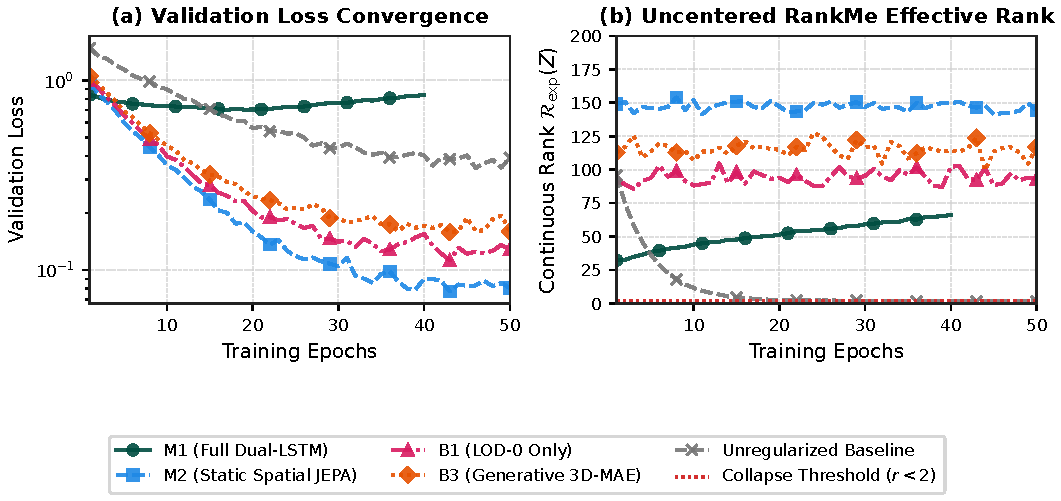
\includegraphics[width=0.92\textwidth]{paper_figs/final/fig1.pdf}
\caption{Pre-training loss convergence and uncentered RankMe effective dimensionality across 50 epochs}
\label{fig:training}
% ALT-TEXT: Two-panel plot showing log-scale validation loss convergence on the left and uncentered RankMe continuous rank trajectories on the right, contrasting M1, M2, B1, B3, and an unregularized collapsing baseline.
\end{figure}

Fig.~\ref{fig:training}(a) illustrates validation loss trajectories across pre-training epochs. Both \textbf{M1} and \textbf{M2} converge smoothly to validation losses of $\textbf{[TBD]}$ and $\textbf{[TBD]}$, respectively. In Fig.~\ref{fig:training}(b), we contrast the uncentered RankMe dimensionality of our VICReg-regularized models against an unregularized baseline. Without variance and covariance penalties, representations collapse rapidly below the effective rank threshold $\mathcal{R}_{\text{exp}} < 2.0$. Conversely, the Spatial JEPA objective sustains stable dimensionalities throughout optimization without dimensional degeneration.

\begin{figure}[t]
\centering
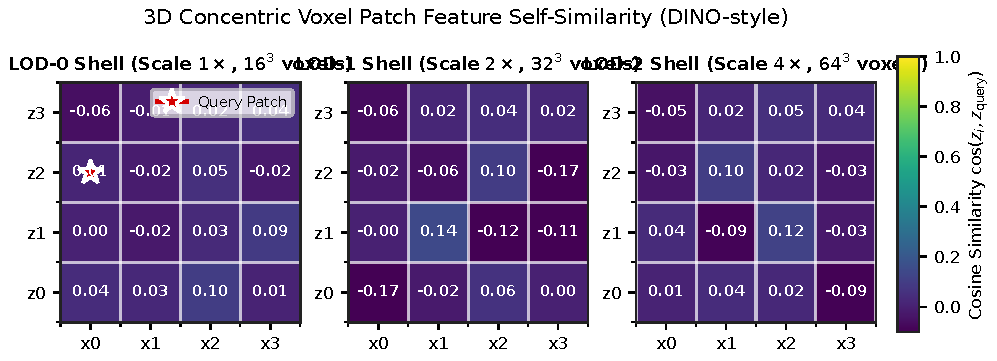
\includegraphics[width=0.92\textwidth]{paper_figs/final/fig2.pdf}
\caption{3D voxel patch cosine similarity maps across concentric LOD shells centered on a query patch}
\label{fig:similarity}
% ALT-TEXT: Multi-panel 3D voxel patch cosine similarity visualization illustrating DINO-style attention localization across LOD-0, LOD-1, and LOD-2 concentric shells.
\end{figure}

To probe spatial clustering in latent space, Fig.~\ref{fig:similarity} visualizes DINO-style cosine similarity maps across all 192 tokens against a selected query patch located in LOD-0~\cite{caron2021dino}. The learned representations exhibit sharp spatial locality within the near-field shell and coherent semantic correspondence extending into outer shells, verifying that cross-scale complementary masking binds multi-resolution features into a unified coordinate frame.

\subsection{Closed-Loop Navigation and Compute Efficiency}

\begin{table}[t]
\centering
\caption{Closed-loop navigation performance and compute profiling in VoxelNavEnv}
\label{tab:navigation}
\begin{tabular}{l c c c c c}
\toprule
\textbf{Policy / Architecture} & \textbf{SR (\%)} & \textbf{SPL} & \textbf{Avg Steps} & \textbf{MFLOPs/step} & \textbf{Latency (ms)} \\
\midrule
\textbf{M1} Dense (Full Temporal) & \textbf{[TBD]} & \textbf{[TBD]} & \textbf{[TBD]} & 1743.6 & \textbf{[TBD]} \\
\textbf{M1} Gated ($\tau_{\text{gate}}=0.05$) & \textbf{[TBD]} & \textbf{[TBD]} & \textbf{[TBD]} & \textbf{[TBD]} & \textbf{[TBD]} \\
\textbf{M2} (Static Spatial JEPA) & \textbf{[TBD]} & \textbf{[TBD]} & \textbf{[TBD]} & 1743.6 & \textbf{[TBD]} \\
\textbf{B1} (Single-LOD0 JEPA)    & \textbf{[TBD]} & \textbf{[TBD]} & \textbf{[TBD]} & 1487.2 & \textbf{[TBD]} \\
\textbf{B2} (Single-LOD2 JEPA)    & \textbf{[TBD]} & \textbf{[TBD]} & \textbf{[TBD]} & 1487.2 & \textbf{[TBD]} \\
\textbf{B3} (Generative 3D-MAE)   & \textbf{[TBD]} & \textbf{[TBD]} & \textbf{[TBD]} & 1743.6 & \textbf{[TBD]} \\
\bottomrule
\end{tabular}
\end{table}

Table~\ref{tab:navigation} presents closed-loop navigation results on complex test courses. Benefiting from temporal integration and ego-motion compensation, \textbf{M1} achieves the highest success rate ($\text{SR} = \textbf{[TBD]}\%$) and path efficiency ($\text{SPL} = \textbf{[TBD]}$). Static \textbf{M2} incurs occasional navigational loops after abrupt turning maneuvers due to lack of recurrent memory ($\text{SR} = \textbf{[TBD]}\%$). The single-scale baseline \textbf{B1} suffers from spatial myopia, failing to orient toward distant goals and stalling at $\text{SR} = \textbf{[TBD]}\%$. Conversely, \textbf{B2} suffers from coarse resolution blindspots, frequently falling off 1-block bridges into lava ($\text{SR} = \textbf{[TBD]}\%$).

\begin{figure}[t]
\centering
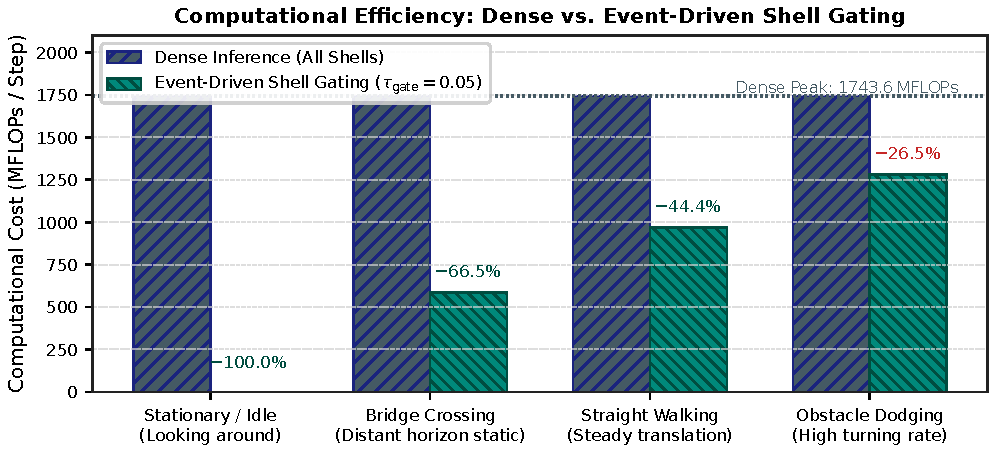
\includegraphics[width=0.88\textwidth]{paper_figs/final/fig3.pdf}
\caption{Inference computational cost comparison between Dense evaluation and Event-Driven Shell Gating ($\tau_{\text{gate}} = 0.05$) across motion regimes}
\label{fig:gating}
% ALT-TEXT: Grouped bar chart comparing computational cost in MFLOPs per step between Dense execution and Event-Driven Shell Gating across Idle, Pitch-Only, Straight Walk, and Active Turning regimes.
\end{figure}

Fig.~\ref{fig:gating} compares the computational cost of dense model evaluation ($1743.6\text{ MFLOPs/step}$) against Event-Driven Shell Gating ($\tau_{\text{gate}} = 0.05$) across diverse motion regimes. When the agent is idle, all three shells fall below threshold, enabling a complete bypass of both 3D CNNs and the Transformer ($0.0\text{ MFLOPs}$, $100\%$ reduction). During straight-line walking, LOD-2 changes negligibly, achieving an average compute saving of $\textbf{[TBD]}\%$. Averaged across comprehensive navigation courses, Event-Driven Gating reduces compute to $\textbf{[TBD]}\text{ MFLOPs/step}$ without degrading navigation success.

\subsection{Latent Space Visualization and Trajectory Analysis}

\begin{figure}[t]
\centering
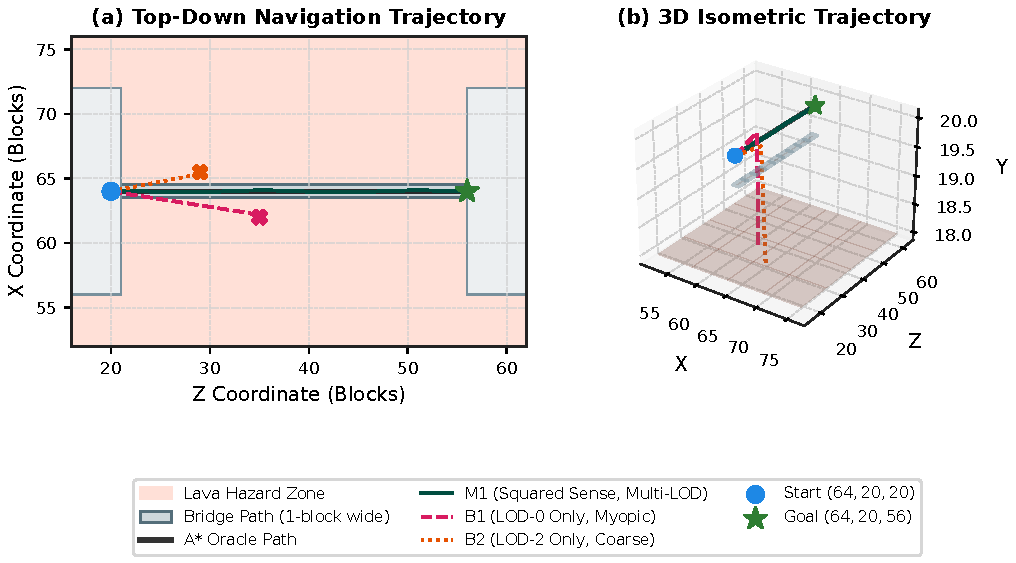
\includegraphics[width=0.92\textwidth]{paper_figs/final/fig4.pdf}
\caption{Overhead top-down and 3D isometric navigation trajectories on the narrow bridge obstacle course}
\label{fig:trajectories}
% ALT-TEXT: Two-panel navigation trajectory plot showing a 2D top-down map and 3D isometric view comparing A-star oracle path against M1, B1, and B2 trajectories over a narrow lava bridge.
\end{figure}

Fig.~\ref{fig:trajectories} visualizes qualitative agent trajectories navigating a narrow 1-block stone bridge suspended over lava. The optimal path is demarcated by an A* oracle. Full Squared Sense (\textbf{M1}) negotiates the bridge with minimal lateral wobble, tracking waypoints safely to the terminal goal $(64, 20, 56)$. In contrast, the myopic single-scale agent \textbf{B1} drifts off course due to absence of distant reference anchors, plunging into lava at $Z = 34$. The coarse agent \textbf{B2} fails to register the exact edge boundary due to spatial downsampling, colliding with hazard boundaries at $Z = 28$. These trajectories directly demonstrate the necessity of multi-scale concentric perception.

\section{Conclusion and Future Work}
In this paper, we introduced Squared Sense, a multi-scale 3D voxel world model designed for efficient, self-supervised spatial intelligence. By structuring egocentric observations into concentric multi-LOD voxel shells, Squared Sense resolves the conflict between spatial horizon and fine resolution under strict volumetric budgets. Our Siamese 3D ConvNeXt encoder and Pre-LN Transformer, pre-trained via Spatial JEPA with VICReg regularization, learn rich geometric representations without generative reconstruction. Event-Driven Shell Gating reduces inference FLOPs by skipping redundant outer-shell evaluations, while the Dual-LSTM temporal integrator tracks dynamic physical state via differentiable 3D ego-motion shift and query cross-attention.

\paragraph{Limitations.} While effective within our discrete-action simulated environment, the current architecture has not yet been deployed on continuous mouse-look actuation in live multiplayer servers. Furthermore, the temporal integrator operates under a single discrete recurrent clock ($5\text{ Hz}$), which may limit multi-timescale credit assignment across extended episodes.

\paragraph{Future Work.} To address these limitations, our direct sequel will explore \textbf{Spatio-Temporal H-JEPA}, coupling concentric spatial shells with hierarchical multi-clock temporal predictors to model long-horizon hierarchical plans in open-world embodied environments.

\subsubsection*{Acknowledgments.}
The authors thank the open-source JAX and Flax developer communities for foundational software tooling. Aryan Mishra is supported in part by graduate research fellowships.

\bibliographystyle{spbasic_unsrt}
\bibliography{references}

\end{document}
